%%%%%%%%%%%%%%%%%%%%%%%%%%%%%%%%%%%%%%%%%
% American Geophysical Union (AGU)
% LaTeX Template
% Version 1.0 (3/6/13)
%
% This template has been downloaded from:
% http://www.LaTeXTemplates.com
%
% Original author:
% The AGUTeX class and agu-ps referencing style were created and are owned 
% by AGU: http://publications.agu.org/author-resource-center/author-guide/latex-formatting-toolkit/
%
% This template has been modified from the blank AGU template to include
% examples of how to insert content and drastically change commenting. The
% structural integrity is maintained as in the original blank template.
%
% Important notes: 
% This template retains extensive commenting from the AGU template. It is heavily 
% advised you read these comments and follow them in order to insure a speedy 
% submission process.
%
%%%%%%%%%%%%%%%%%%%%%%%%%%%%%%%%%%%%%%%%%

%%%%%%%%%%%%%%%%%%%%%%%%%%%%%%%%%%%%%%%%%%%%%%%%%%%%%%%%%%%%%%%%%%%%%%%%%%%%
% AGUtmpl.tex: this template file is for articles formatted with LaTeX2e,
% Modified March 2013
%
% This template includes commands and instructions
% given in the order necessary to produce a final output that will
% satisfy AGU requirements.
%
% PLEASE DO NOT USE YOUR OWN MACROS
% DO NOT USE \newcommand, \renewcommand, or \def.
%
% FOR FIGURES, DO NOT USE \psfrag or \subfigure.
%
%%%%%%%%%%%%%%%%%%%%%%%%%%%%%%%%%%%%%%%%%%%%%%%%%%%%%%%%%%%%%%%%%%%%%%%%%%%%
%
% All questions should be e-mailed to latex@agu.org.
%
%%%%%%%%%%%%%%%%%%%%%%%%%%%%%%%%%%%%%%%%%%%%%%%%%%%%%%%%%%%%%%%%%%%%%%%%%%%%

% Step 1: Set the \documentclass

% There are two options for article format: two column (default) and draft.

% PLEASE USE THE DRAFT OPTION TO SUBMIT YOUR PAPERS.
% The draft option produces double spaced output.

% Choose the journal abbreviation for the journal you are submitting to:

% jgrga	JOURNAL OF GEOPHYSICAL RESEARCH
% gbc	GLOBAL BIOCHEMICAL CYCLES
% grl		GEOPHYSICAL RESEARCH LETTERS
% pal	PALEOCEANOGRAPHY
% ras	RADIO SCIENCE
% rog	REVIEWS OF GEOPHYSICS
% tec	TECTONICS
% wrr	WATER RESOURCES RESEARCH
% gc		GEOCHEMISTRY, GEOPHYSICS, GEOSYSTEMS
% sw	SPACE WEATHER
% ms	JAMES
%
%
%
% (If you are submitting to a journal other than jgrga,
% substitute the initials of the journal for "jgrga" below.)

\documentclass[two column,grl]{AGUTeX}

% To create numbered lines:


% If you don't already have lineno.sty, you can download it from http://www.ctan.org/tex-archive/macros/latex/contrib/ednotes/ (or search the internet for lineno.sty ctan), available at TeX Archive Network (CTAN). Take care that you always use the latest version.

% To activate the commands, uncomment \usepackage{lineno} and \linenumbers*[1]command, below:

%\usepackage{lineno}
%\linenumbers*[1]
%\usepackage{natbib}
%  To add line numbers to lines with equations:
%  \begin{linenomath*}
%  \begin{equation}
%  \end{equation}
%  \end{linenomath*}

%%%%%%%%%%%%%%%%%%%%%%%%%%%%%%%%%%%%%%%%%%%%%%%%%%%%%%%%%%%%%%%%%%%%%%%%%
% Figures and Tables

% DO NOT USE \psfrag or \subfigure commands.

%  Figures and tables should be placed AT THE END OF THE ARTICLE, after the references.

%  Uncomment the following command to include .eps files (comment out this line for draft format):

\usepackage{graphicx}
\usepackage{epstopdf}
\usepackage{epsfig}

% Substitute one of the following for [dvips] above if you are using a different driver program and want to proof your illustrations on your machine:
% [xdvi], [dvipdf], [dvipsone], [dviwindo], [emtex], [dviwin],
% [pctexps],  [pctexwin],  [pctexhp],  [pctex32], [truetex], [tcidvi],
% [oztex], [textures]

%  Uncomment the following command to allow illustrations to print when using Draft:
\setkeys{Gin}{draft=false}

% See how to enter figures and tables at the end of the article, after references.

%----------------------------------------------------------------------------------------
%	RUNNING HEAD AND CORRESPONDING AUTHOR
%----------------------------------------------------------------------------------------

% Author names in capital letters:
\authorrunninghead{NGUYEN ET AL.}

%------------------------------------------------

% Shorter version of title entered in capital letters:
\titlerunninghead{METHANE EMISSIONS ESTIMATES}

%------------------------------------------------

% Corresponding author mailing address and e-mail address:
\authoraddr{: Newton Nguyen, Department of Environmental Science and Engineering, California Institute of Technology, Pasadena, California, USA. (newton@caltech.edu)}

%----------------------------------------------------------------------------------------

\begin{document}

%----------------------------------------------------------------------------------------
%	TITLE
%----------------------------------------------------------------------------------------

\title{Effects of Interactive Hydroxyl Chemistry on Decadal Methane Emissions Estimates}

%----------------------------------------------------------------------------------------
%	AUTHORS AND AFFILIATIONS
%----------------------------------------------------------------------------------------

% Use \author{\altaffilmark{}} and \altaffiltext{}

% \altaffilmark will produce footnote; matching \altaffiltext will appear at bottom of page.

\authors{Newton Nguyen,\altaffilmark{1}}
%James Smith,\altaffilmark{1,2}, and
%Jane Smith\altaffilmark{2}}


\altaffiltext{1}{Department of Environmental Science and Engineering, California Institute of Technology, Pasadena, California, USA.}

%----------------------------------------------------------------------------------------
%	ABSTRACT
%----------------------------------------------------------------------------------------

% Do NOT include any \begin...\end commands within the body of the abstract.

\begin{abstract}

The rise of atmospheric methane experienced a brief pause between 2000 and 2007 with a subsequent resumption in growth continuing to the present day. Questions on both the commencement and termination of this stabilization remain open due to uncertainty in methane sources and its main sink, reaction with the hydroxyl radical (OH). In the atmosphere, methane undergoes oxidation reactions and thus, its lifetime depends on the concentration of hydroxyl radicals. Methyl Chloroform has been used to constrain global hydroxyl concentrations and infer methane lifetimes. Here, we report on results using a two-hemispheres box model that includes dynamic chemistry of methane, carbon monoxide, and the hydroxyl radical. We will discuss the impact of critical assumptions on methane flux inversions: 1) Constant OH concentrations and 2) Constant OH sources with interactive chemistry assuming constant or variable CO, 3) variable OH sources, 4) variations in OH inter-hemispheric gradients. Hemispheric sources are calculated from a nonlinear, stochastic Bayesian inversion constrained by data from methane (NOAA), carbon monoxide (NOAA), and Methyl chloroform (NOAA, GAGE/AGAGE) observations. We perform sensitivity experiments by calculating the impact that including each aspect of the chemical system has on the emissions estimates. Based on our results, we find that when ignoring interactive OH chemistry, methane emissions have a negative bias at the beginning of the 21st century, during negative OH anomalies. However, when CO emissions are accounted for, the reduction in CO emissions beginning in the 1990’s results in increasing methane emissions but relatively higher OH concentrations; this is due to CO emissions decreasing during this period. We also find that when account for a variable OH source, our results agree with those found in \citep{turner_ambiguity_2017}.
\end{abstract}

%----------------------------------------------------------------------------------------
%	ARTICLE CONTENT
%----------------------------------------------------------------------------------------

% The body of the article must start with a \begin{article} command
% \end{article} must follow the references section, before the figures and tables.

\begin{article}

\section{Introduction}
The steady rise of methane concentrations in the Earth’s atmosphere was interrupted by a brief stabilization from 2000 to 2007 with  a subsequent resumption in growth; the causes of the onset and renewed growth remain ambiguous. Overall, methane concentrations have tripled  from 750 ppb in 1850 to 1850 ppb in the present day \citep{IPCC}. Methane is not only the second most important anthropogenic greenhouse gas  but also a  precursor to tropospheric ozone, itself a greenhouse gas and air pollutant \citep{fiore_impact_2006, shindell_simultaneously_2012, IPCC}. Its sources are spatially and temporally heterogeneous and its sinks can also be  variable, resulting in major uncertainties in determining the cause of the stabilization.

\begin{figure}
\begin{center}
\includegraphics[width= 0.45\textwidth]{./methane_timeseries.png}
\end{center}
\caption{Plotted is a timeseries of methane concentrations collected through ice core measurements from the last ~2,000 years. On the right, decadal scale concentrations are shown with focus on the Methane Stabilization.}
\end{figure}

Changes in methane sources have been proposed as possible explanations for the cause of the renewed growth. Major sources include microbial production in wetlands, permafrost melting in the high latitudes, biomass burning, rice cultivation, solid and liquid waste, and activities related to fossil fuel extraction. A shift in global $\delta^{13}C$ towards more depleted carbon indicates that the end of the stabilization could have been driven by a change in methane sources \citep{bousquet_contribution_2006, kai_reduced_2011}. 

Biogenic sources favor lighter C and a shift towards more depleted $\delta^{13}C$ can indicate either an increase in isotopically lighter, e.g. biogenic, sources or a decrease in heavier, e.g. pyrogenic and thermogenic, sources \citep{nisbet_rising_nodate, schaefer2016}. An analysis by \citep{nisbet_rising_nodate} concludes that a shift towards lighter isotopes demonstrate an increase in wetland emissions, while \citep{schaefer2016} conclude that the isotopic shift is due to increased emissions from agricultural production. Yet, the change in the isotopic composition can also have been caused by a decrease in biomass burning sources, which are isotopically heavy, alongside an increase in fossil fuel sources, which are generally lighter than biomass burning sources and heavier than biogenic sources; \citep{worden_reduced_2017} concludes this. These studies came to different conclusions with the same constraints indicating that the problem may be underdetermined.

Other studies have focused on a change in the methane sink. Methane loss is primarily driven by oxidation via OH radicals but also transport to the stratosphere, consumption by methanotrophic microbes in soils, and oxidation by chlorine radicals. The Hydroxyl Radical accounts for about 90\% of methane loss and thus is the main mechanism of methane loss in the troposphere. \citep{turner_ambiguity_2017} and \citep{rigby_role_2017}, using Methyl Chloroform (MCF) as a proxy for Hydroxyl Radical concentrations, conclude that changes in hydroxyl concentrations occurred during the stabilization period. Yet, their conclusions differ. \citep{rigby_role_2017} conclude that a decline in Hydroxyl concentrations accompanied by a slow-down in the methane growth rate was implicated in the renewed growth, while \citep{turner_ambiguity_2017} find that the renewed growth was caused by a decline in Hydroxyl radicals with a decrease in methane emissions. Yet, a causal mechanism for a decrease in hydroxyl concentrations has not been found. Quantifying the effect of dynamical Hydroxyl concentrations on methane emissions estimates provides a useful constraint on the methane stability problem.

The relationship between methane concentrations and emissions is nonlinear; this increases the complexity of the system and makes emissions estimates more difficult. Methane is a short lived greenhouse gas with a lifetime of approximately a decade. However, it’s lifetime primarily depends on the concentration of the Hydroxyl Radical, e.g. higher concentrations of OH results in a shorter methane lifetime. In addition, the oxidation of methane yields carbon monoxide which also consumes hydroxyl radicals \citep{prather_lifetimes_2007}. Previous studies use MCF to constrain methane lifetime \citep{rigby_role_2017, turner_ambiguity_2017}. We instead account for variable methane lifetime by including dynamic CH4, CO, and OH chemistry in our model. The objective of the present study is to quantify the systematic biases when including (excluding) variable methane lifetimes and thus interactive chemistry in the estimation of emissions.

Here, we include interactive methane chemistry in our inversions by using a two hemispheres box model with CH4, CO, and OH chemistry. We will discuss the impact of critical assumptions on methane flux inversions: 1) Constant OH concentrations and 2) Constant OH sources with interactive chemistry assuming constant or variable CO, 3) variable OH sources, 4) variations in OH inter-hemispheric gradients. Section 2 provides the theoretical background for the variability of methane lifetimes, Section 3 describes the model and data employed in the current study, and in Section 4, we discuss the conclusions of the study and provide recommendations for future work in methane emissions estimates over the decadal timescale.


%------------------------------------------------

\section{Theoretical Background and Forward Model}
We use the model developed by \citep{prather_time_1996, prather1994lifetimes} in the developement of our forward model. In the atmosphere, the hydroxyl radical is the primary mechanism of methane loss. 
\begin{equation}
    OH + CH_4 \Longrightarrow (multiple steps) \Longrightarrow CO + products \\
\end{equation}
CO is the largest sink of OH in the troposphere and thus, the concentration of OH depends on both the concentrations of CH4 and CO.
\begin{equation}
    OH + CO \Longrightarrow CO_2 + H 
\end{equation}
In addition, the hydroxyl radical also reacts with other compounds in the atmosphere such as ethane, propane, and other non methane hydrocarbons in addition to being recycled with the emission of NOx. Therefore, we create another OH loss reaction that abstracts this complexity with an arbitrary group of molecules X \citep{prather_time_1996, prather1994lifetimes}.
\begin{equation}
    OH + X \Longrightarrow products 
\end{equation}
These reactions form the OH loss terms in our box model. From these reactions and their kinetics, we can form a set of coupled differential equations:

\begin{eqnarray}
    R_1 &= k_1 [OH] [CH_4] \\ 
    R_2 &= k_2 [OH] [CO] \\
    R_3 &= k_3 [OH] [X] \\
    \frac{d[CH_4]}{dt} &= SCH_4 - R_1 - \frac{\Delta[CH_4]}{\tau}\\
    \frac{d[CO]}{dt} &= SCO + R_1 - R_2 - \frac{\Delta[CO]}{\tau}\\
    \frac{d[OH]}{dt} &= SOH - R_1 - R_2 - R_3 - \frac{\Delta[OH]}{\tau}
  \end{eqnarray}

Above, $\Delta[c]$ is the difference in the concentration of species $c$ between the Northern and Southern Hemispheres, $\tau$ is the inter hemispheric exchange timescale, ~1 yr, and hence, $\Delta[c]/\tau$ is the inter hemispheric transport term. Finally, $S_c$ is the source term which represents the emission of the species $c$ and in the case of OH, represents the production rate. These equations are computed in our forward model. \\

As a test of our forward model, we run the model with prescribed emissions. We then add a 50% instantaneous perturbation to methane emissions and observe the behavior of the system with interactive and noninteractive OH chemistry Fig. \ref{forward_model}. the perturbation lifetime of the non interactive chemistry model decays with a ~9 yr lifetime while the interactive chemistry decays with a ~13 yr lifetime. This is expected \citep{prather_time_1996, prather1994lifetimes} and indicates that our forward model is accurately approximating the chemical system to first order. 

\begin{figure} \label{forward_model}
\begin{center}
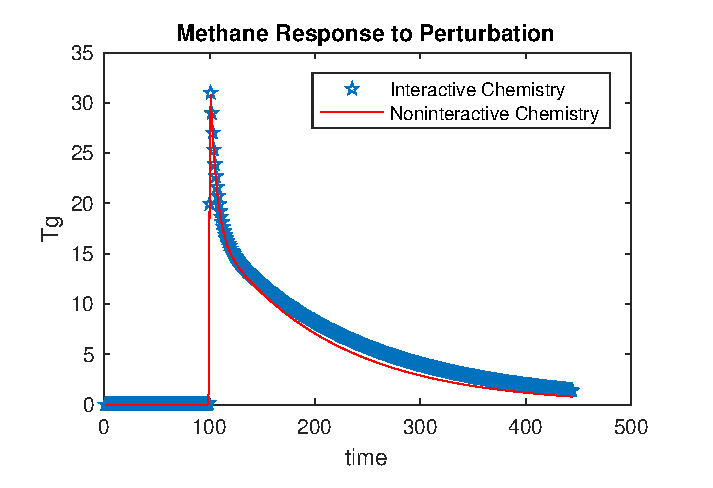
\includegraphics[width=0.5\textwidth]{forward_model_test.eps}
\end{center}
\end{figure}


%% Maybe have the MCF equation instead of OH 
%------------------------------------------------

\section{Methods}
\subsection{Data and Inversion}
Our box model (section 2) maps emissions to concentrations and thus, by inverting our model, we map concentrations to emissions. Emissions are estimated using a nonlinear bayesian inversion method, the Levenberg-Marquardt algorithm. We use observations of methane (NOAA), carbon monoxide (NOAA), and Methyl chloroform (NOAA, GAGE/AGAGE) concentrations.

Concentration measurements began in 1983 and continue into the present day. For our inversions, we take hemispheric averages by bootstrapping the deseasonalized data. These observations are combined by block averaging in 1 yr windows to form a timeseries. This process is repeated 50 times so that the mean and variance of these timeseries can be calculated. The data are then inputted into our inversion and emissions are derived by minimizing the cost function with our box model as the forward model.


\subsection{Simulations}
We first perform an idealized inversion test by globally prescribing fixed emissions until an arbitrary year and prescribe an increase emissions by 20 Tg/yr in our forward model with interactive OH chemistry. The resulting concentrations are inverted for emissions in two different runs where we A), assume non interactive OH chemistry and B), assume interactive OH chemistry. This test serves two purposes: 1), We can test the performance of our inversion and 2), we can calculate the error when concentrations, calculated with interactive OH chemistry, are inverted for emissions while neglecting interactive OH chemistry. This is equivalent to computing the forward model error of using a simple fixed OH concentration in atmospheric methane inversions, which is common practice.

From the results of our Synthetic Emissions Test, Fig. \ref{synthetic_emissions}, we find that the forward model error when not accounting for interactive OH chemistry is in close agreement with the prescribed emissions. This implies our inversion is accurately solving for emissions despite the added complexity to the forward model. However, the inversion without interactive OH chemistry begins changing sign when the prescribed emissions spike begins Fig. \ref{synthetic_emissions}. This is due to the fact that increased Methane emissions decrease Hydroxyl concentrations. The noninteractive OH inversion does not account for this OH concentration response and results in an underestimation in an atmosphere with higher OH concentrations and an overestimation in an atmosphere with lower OH concentrations. This is discussed further in Section 4. 

\begin{figure*} \label{synthetic_emissions}
\begin{center}
\includegraphics[width=\textwidth]{synthetic_emissions_test.eps}
\end{center}
\caption{A test of our inversion. We prescribe emissions and increase it by 20 Tg/yr to test our inversion. We then run our inversion with interactive OH chemistry and non interactive OH chemistry}
\end{figure*}

In addition, we run our inversions with increasing levels of complexity in order to obtain the biases associated with including (excluding) interactive OH chemistry and carbon monoxide in emissions estimates. \ref{model_setup} shows the model runs. In our experiments, Case 1, our simplest run, assumes fixed OH concentrations (non interactive chemistry). Case 2 assumes fixed CO and OH sources with interactive chemistry while Case 3 accounts for the temporal variability of CO sources. Case 4 incorporates the variability of OH sources without variable CO sources while Case 5 accounts for the temporal variability of CO sources with variable OH sources. The results of thes runs are plotted in Fig. \ref{all_runs}.


\begin{table} \label{model_setup}
\caption{Our simulations vary in complexity. Below are the assumptions in each model run.}
\begin{tabular}{| c | c| c| c|}
Case & Interactive OH & Inverting with CO & Inverting for OH Source \\ \hline
1 &  no & no & no  \\
2 & yes & no & no \\
3 & yes & yes & no \\
4 & yes & no & yes \\
5 & yes & yes & yes 
\end{tabular}
\end{table}


\begin{figure*} \label{all_runs}
\begin{center}
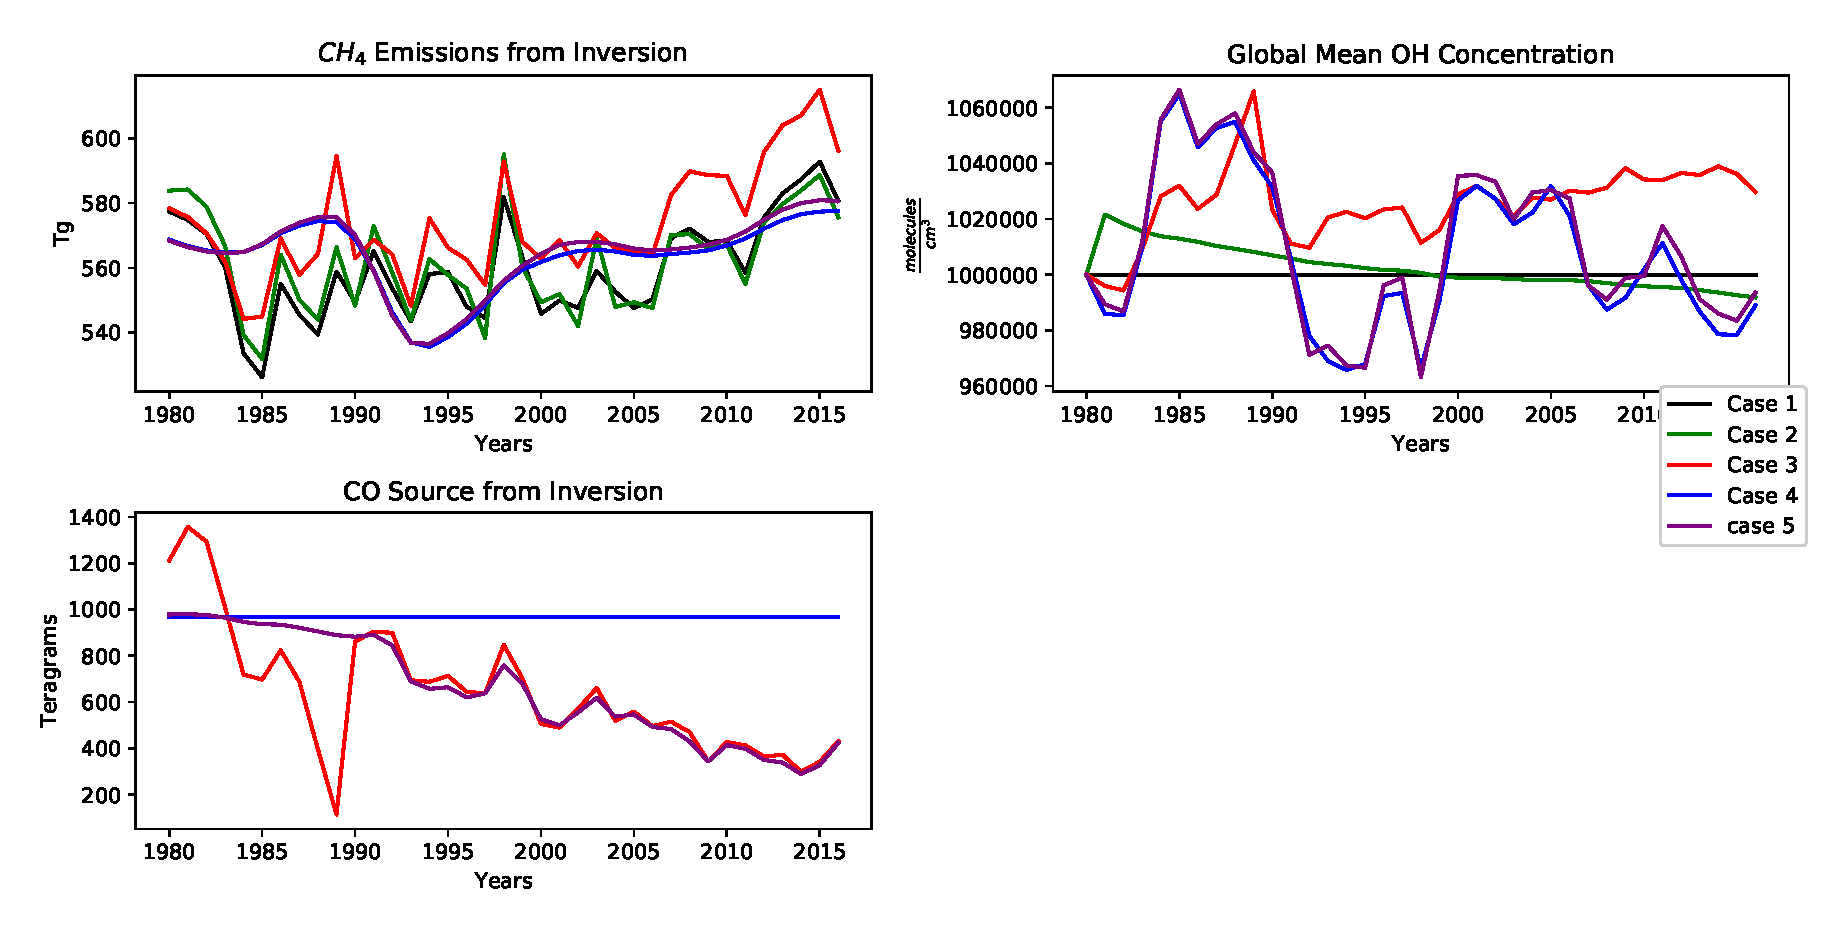
\includegraphics[width=\textwidth]{case_emissions.eps}
\end{center}
\caption{Plotted are the results from our inversion for all five cases in Table 1. Calculated methane emissions are on the top left panel, CO emissions are on the top right panel, and OH concentrations are on the bottom left panel.}
\end{figure*}


%------------------------------------------------

\section{Discussion}

In this study, we estimated global methane emissions in a 2 hemispheres box model and quantify the biases associated with critical assumptions in decadal methane emissions estimates between the years 1980 to 2016 (Table 1). When excluding interactive OH chemistry, (fig. xx), our results indicate a bias that depends on the availability of OH radicals in the atmosphere.. When not accounting for interactive OH chemistry, higher OH concentrations result in a negative bias and low OH concentrations result in a positive bias. This can be seen in Fig xx where increased methane emissions at the turn of the century decrease the amount of OH radicals and an overestimation of emissions (Fig. \ref{OH_bias}). In case 1, with fixed OH concentrations, methane emissions increase by 6.6\% between 1996 and 2016.  In case 2, methane emissions increase by 6.9\% while global mean OH concentrations decrease by 0.95\%.

\begin{figure*} \label{OH_bias}
\begin{center}
\includegraphics[width=\textwidth]{OH_variability_bias.eps} \\
\end{center}
\caption{ Above are inversion results from ignoring interactive OH chemistry (Case 1) and accounting for interactive OH chemistry with assuming a fixed CO emission (Case 2). The left panel shows calculated emissions from 1980 to 2016. The right panel shows the difference in $CH_4$ emissions with the assumptions outlined in Table 1.}
\end{figure*}

when CO emissions are increasing before the 1990’s, increased emissions caused a decrease in OH concentration and a reduced estimation of methane emissions. However, with the decrease in CO emissions beginning in the 1990’s, we see an increased availability of OH radicals to oxidize Methane, and hence, decreasing Methane lifetime results in increasing Methane emissions to match observations (Fig. \ref{CO_bias} \ref{all_runs}. In case 3, global methane emissions increase by 7.4\% with a decrease in OH concentrations by 0.5\% between 1996 and 2016. This indicates that the reduction in CO more than compensates for the increased methane emissions in OH loss. 

\begin{figure*} \label{CO_bias}
\begin{center}
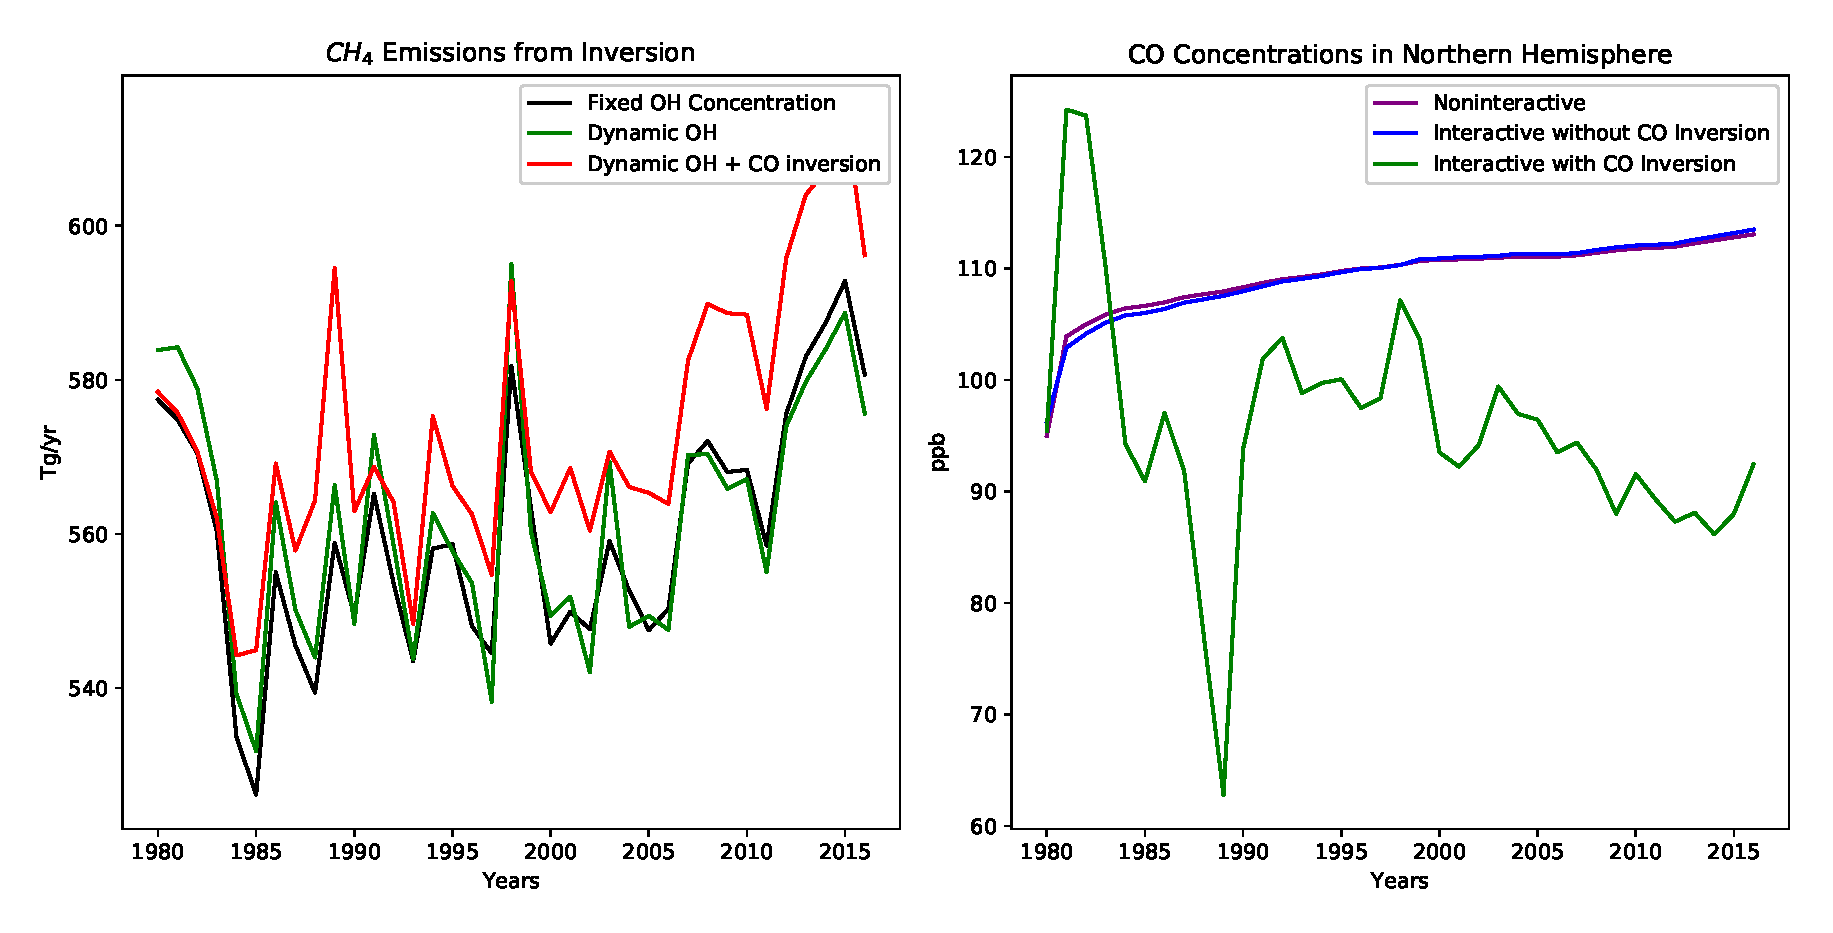
\includegraphics[width=\textwidth]{CO_bias.eps}
\end{center}
\caption{Plotted are the results from our inversion for cases 1-3. Methane emissions are on the left panel and CO concentrations are on the right panel.}
\end{figure*}

In Case 4 and Case 5, we additionally fit for variability in the OH production rate. Case 4 assumes constant CO emissions while Case 5 accounts for the variability of CO emissions. The differences between Methane emissions in both cases is small. They also generally agree with the solution obtained by \citep{turner_ambiguity_2017}. 

In summary, we find that not accounting for interactive OH chemistry and the variability of CO emissions biases the results of methane emissions estimates in opposing ways. Methane lifetime depends on the concentration of the Hydroxyl Radical which, in turn, depends on the concentration of CO and CH4. In decadal Methane emissions estimates, we find a systematic negative bias in inversions that do not account for this chemical system. This is due to the decline of CO emissions starting in the 1990’s overcompensating for the loss of OH due to CH4. However, when allowing for a varying OH source term, our results match that of \citep{turner_ambiguity_2017} because of compensating OH production accounting for variabilities in OH concentrations due to interactive chemistry. 

We conclude that future work in estimating methane emissions in the decadal timescale should account for the interactive OH chemistry that takes place in the troposphere, and more work should be done to constrain trends in the concentration and production of Hydroxyl radicals due to its effect on the methane lifetime. 




%----------------------------------------------------------------------------------------
%	ACKNOWLEDGEMENTS
%----------------------------------------------------------------------------------------

\begin{acknowledgments}
Many thanks to Christian Frankenberg, Alex Turner, and Yi Yin for the invaluable assistance in preparing this project. 
\end{acknowledgments}
\bibliography{citations}{}
\bibliographystyle{apalike}

%----------------------------------------------------------------------------------------
%	BIBLIOGRAPHY
%----------------------------------------------------------------------------------------

% Either type in your references using
% \begin{thebibliography}{}
% \bibitem{}
% Text
% \end{thebibliography}

% Or,

% If you use BiBTeX for your references, please use the agufull08.bst file (available at % ftp://ftp.agu.org/journals/latex/journals/Manuscript-Preparation/) to produce your .bbl
% file and copy the contents into your paper here.

% Follow these steps:
% 1. Run LaTeX on your LaTeX file.

% 2. Make sure the bibliography style appears as \bibliographystyle{agufull08}. Run BiBTeX on your LaTeX
% file.

% 3. Open the new .bbl file containing the reference list and
%   copy all the contents into your LaTeX file here.

% 4. Comment out the old \bibliographystyle and \bibliography commands.

% 5. Run LaTeX on your new file before submitting.

% AGU does not want a .bib or a .bbl file. Please copy in the contents of your .bbl file here.


\end{article}

%----------------------------------------------------------------------------------------
%	FIGURES AND TABLES
%----------------------------------------------------------------------------------------

%% Enter Figures and Tables here:
%
% DO NOT USE \psfrag or \subfigure commands.
%
% Figure captions go below the figure.
% Table titles go above tables; all other caption information should be placed in footnotes below the table.
%
%----------------
% EXAMPLE FIGURE
%
% \begin{figure}
% \noindent\includegraphics[width=20pc]{samplefigure.eps}
% \caption{Caption text here}
% \label{figure_label}
% \end{figure}
%
% ---------------
% EXAMPLE TABLE
%
%\begin{table}
%\caption{Time of the Transition Between Phase 1 and Phase 2\tablenotemark{a}}
%\centering
%\begin{tabular}{l c}
%\hline
% Run  & Time (min)  \\
%\hline
%  $l1$  & 260   \\
%  $l2$  & 300   \\
%  $l3$  & 340   \\
%  $h1$  & 270   \\
%  $h2$  & 250   \\
%  $h3$  & 380   \\
%  $r1$  & 370   \\
%  $r2$  & 390   \\
%\hline
%\end{tabular}
%\tablenotetext{a}{Footnote text here.}
%\end{table}

% See below for how to make sideways figures or tables.

\newpage





\end{document}



% IF YOU HAVE MULTI-LINE EQUATIONS, PLEASE
% BREAK THE EQUATIONS INTO TWO OR MORE LINES
% OF SINGLE COLUMN WIDTH (20 pc, 8.3 cm)
% using double backslashes (\\).

% To create multiline equations, use the
% \begin{eqnarray} and \end{eqnarray} environment
% as demonstrated below.

%If you don't want an equation number, use the star form:
%\begin{eqnarray*}...\end{eqnarray*}

% Break each line at a sign of operation
% (+, -, etc.) if possible, with the sign of operation
% on the new line.

% Indent second and subsequent lines to align with the first character following the equal sign on the first line.

% Use an \hspace{} command to insert horizontal space into your equation if necessary. Place an appropriate unit of measure between the curly braces, e.g. \hspace{1in}; you may have to experiment to achieve the correct amount of space.


%% ------------------------------------------------------------------------ %%
%
%  EQUATION NUMBERING: COUNTER
%
%% ------------------------------------------------------------------------ %%

% You may change equation numbering by resetting
% the equation counter or by explicitly numbering
% an equation.

% To explicitly number an equation, type \eqnum{}
% (with the desired number between the brackets)
% after the \begin{equation} or \begin{eqnarray}
% command.  The \eqnum{} command will affect only
% the equation it appears with; LaTeX will number
% any equations appearing later in the manuscript
% according to the equation counter.
%

% If you have a multiline equation that needs only
% one equation number, use a \nonumber command in
% front of the double backslashes (\\) as shown in
% the multiline equation above.

%% ------------------------------------------------------------------------ %%
%
%  SIDEWAYS FIGURE AND TABLE EXAMPLES
%
%% ------------------------------------------------------------------------ %%
%
% For tables and figures, add \usepackage{rotating} to the paper and add the rotating.sty file to the folder.
% AGU prefers the use of {sidewaystable} over {landscapetable} as it causes fewer problems.
%
% \begin{sidewaysfigure}
% \includegraphics[width=20pc]{samplefigure.eps}
% \caption{caption here}
% \label{label_here}
% \end{sidewaysfigure}
%
% \begin{sidewaystable}
% \caption{}
% \begin{tabular}
% Table layout here.
% \end{tabular}
% \end{sidewaystable}
